%%% METHODOLOGY %%%
\section{Methodology} \label{sec:methods}

Professor Vassilis Kalantzis, who we contacted via email, generously provided us with the relevant MATLAB code and data; however, we chose to re-implement the algorithm from scratch in Python with standard packages (NumPy \cite{numpy}, SciPy \cite{scipy}, and scikit-learn \cite{scikit-learn}) and used the MATLAB code to confirm our implementation.
We compared the performance of Algorithms 2.1 and 2.2 with \verb|FrequentDirections| \cite{Ghashami2016}, a state-of-the-art streaming algorithm.
Experiments were conducted on a MacBook Pro with a 2.3 GHz Dual-Core Intel Core i5 processor with 16 GB of RAM, and the code is publicly available on GitHub\footnote{https://anonymous.4open.science/r/truncatedSVD-0162/}.
All plots were generated using Matplotlib \cite{matplotlib}.

%% IMPLEMENTATION
\subsection{Implementation}

We chose to implement the three truncated SVD update algorithms as methods of an \verb|EvolvingMatrix| class, which we will refer to as \verb|EM| from here on out.
With each experiment, the \verb|EM| class was initialized with various parameters (initial matrix, matrix to be appended, number of batches, etc.) and updates were carried out using one of the update methods.
A simplified version of the experiment is shown in Listing \ref{lst:exp_pseudo}.
Algorithms 2.1 and 2.2 were written based on the pseudo-code presented in Algorithm \ref{alg:row-update}, where the $Z$ and $Z^H A$ matrices were calculated using their respective formulas. 

\lstinputlisting[language=python, float, floatplacement=h, caption=Simplified experiment structure, label={lst:exp_pseudo}]{../openreview/sections/exp.py}

\paragraph{Algorithm 2.1}

The $Z$ and $Z^H A$ matrices were constructed as in Equations \ref{eq:zha-simon_Z} and \ref{eq:zha-simon_ZHA}, respectively. 

\paragraph{Algorithm 2.2}

The main difficulty in implementing Algorithm 2.2 was in the calculation of $X_{\lambda,r}$.
We chose to solve for $X$ in Equation \ref{eq:bcg} using the block Conjugate Gradient method (BCG) \cite{OLeary1980} as recommended in \cite{Kalantzis2021}.
Though \cite{Kalantzis2021} specified, at maximum, one iteration of BCG, we found that the MATLAB code set the limit to two iterations.
As the additional iteration did not greatly increase the computational cost, we chose to run BCG a maximum of two iterations as well.
Once $X$ was calculated, we calculated $X_{\lambda,r}$ as per Equation \ref{eq:bcg_rsvd} using randomized SVD \cite{Halko2011}.
For this, we used the scikit-learn \verb|randomized_svd| implementation \cite{scikit-learn}.
Based on the description for calculating $X_{\lambda,r}$ in \cite{Kalantzis2021}, we set \verb|n_components|$=r$, \verb|n_oversamples|$=2r$, and \verb|n_iter|$=0$.
The $X_{\lambda,r}$ returned was then used to calculate $Z$ and $Z^H A$ as in Equations \ref{eq:enhanced_Z} and \ref{eq:enhanced_ZHA}, respectively.

\paragraph{Frequent Directions}

A modified version of \verb|FrequentDirections|\footnote{https://github.com/edoliberty/frequent-directions} was incorporated as an update method into the $\verb|EM|$ class.
Since \verb|FrequentDirections| is a line-by-line update method as opposed to a batch update method, the update method in the $\verb|EM|$ class was constructed to receive a matrix $E$ containing the rows to be added and performs the \verb|FrequentDirections| algorithms for each row of the $E$.
Any form of error metric calculation or subsequent update is performed only after the entire matrix $E$ has been processed using the line-by-line update method.

Since the updated matrix $B$ for the \verb|FrequentDirections| method has constant dimensions throughout the update process, the residual norm error calculation is modified to measure the error between $B$ and $A'$ where $A'$ is a truncated version of $A$ that only holds the first $2l$ singular vectors and values of $A$ and where $2l$ is the number of rows in $B$.

%% DATASETS %%
\subsection{Datasets}

In total, we conducted experiments on five datasets. MED, CRAN, CISI, and Reuters-21578 are term-document matrices from latent semantic indexing applications \cite{LSISite,Cai2005,Cai2007,Cai2008,Cai2009} and ML1M is a movie rating dataset from MovieLens \cite{Harper2015}.
Table \ref{table:datasets} lists the dimensions of the matrices as well as the average number of nonzero (nnz) entries per row and Figure \ref{fig:sv} shows the leading 100 singular values for each matrix.
It should be noted that the matrices used for CISI, CRAN, and MED in \cite{Kalantzis2021} had slightly different dimensions compared to what was listed on \cite{LSISite}.
We received these datasets along with the MATLAB code and chose to use their versions of the data for ease of comparison; as we were interested in the accuracy of singular value reconstruction we determined that somewhat corrupted data merely introduced a different set of singular values to reconstruct.
Furthermore, as the Reuters and ML1M datasets were intact, we used them as controls against the corruption of the other sets.

% Plot of singular value profile plot and table of data matrix stats
\begin{center}
\begin{minipage}[b]{0.4\textwidth}
% \begin{figure}[h]
  \centering
  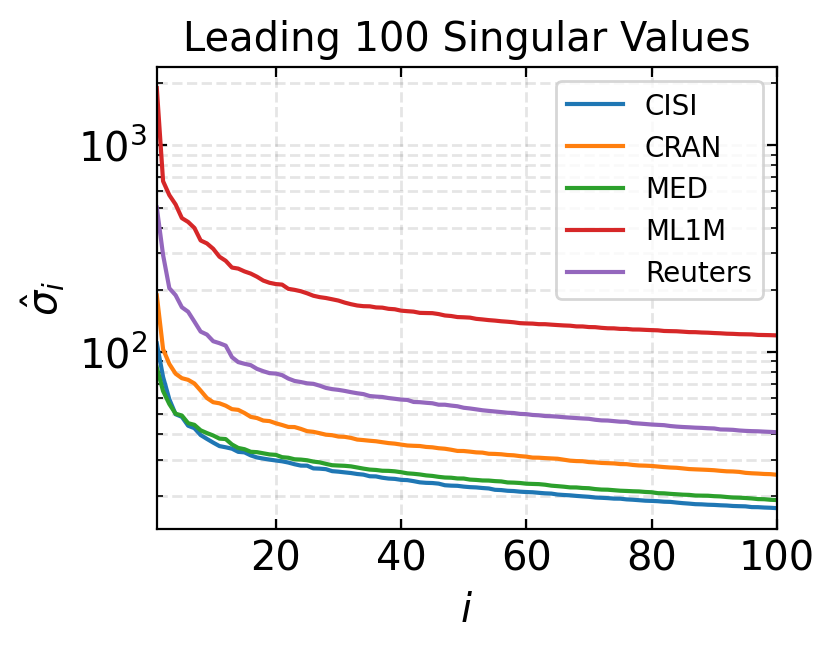
\includegraphics[width=0.9\textwidth]{figures/sv_100_profile.png}
  \captionof{figure}{Leading 100 singular values for each dataset.}
  \label{fig:sv}
% \end{figure}
\end{minipage}
\hfill
\begin{minipage}[b]{0.58\textwidth}
% \begin{table}[h]
  \centering
  \begin{tabular}{cccc}
    \toprule
    Dataset       & Rows  & Columns & nnz(A)/row \\
    \midrule
    CISI \cite{LSISite}                                     & 5609  &    1460 &      12.17 \\
    CRAN \cite{LSISite}                                     & 4612  &    1398 &      18.06 \\
    MED  \cite{LSISite}                                     & 5831  &    1033 &       8.92 \\
    ML1M \cite{Harper2015}                                  & 6040  &    3952 &     165.60 \\
    Reuters-21578 \cite{Cai2005, Cai2007, Cai2008, Cai2009} & 18933 &    8293 &      20.57 \\
    \bottomrule
    \vspace{5mm}
  \end{tabular}
  \\
  \captionof{table}{Number of rows, columns, and average non-zero elements in each row for datasets.}
  \label{table:datasets}
% \end{table}
\end{minipage}
\end{center}

%% EXPERIMENTS %%
\subsection{Experiments}

We conducted two sets of experiments: one to confirm the results of \cite{Kalantzis2021} in a series of reproducibility studies and another to further measure the performance of the algorithms using two additional metrics as well as observing the effect of the number of batches on the runtime and performance.

\paragraph{Update method comparison} 

As a first step, we sought to reproduce the results in Figures 3 and 4 of \cite{Kalantzis2021}.
To do this, we conducted the sequence updates experiment.
The initial matrix $B\equiv A^{(0)}$ was set equal to the first $\mu$ rows of $A\in\Ctwo{m}{n}$ and the remaining $m-\mu$ rows of $A$ were appended to the initial matrix over a sequence of $\phi$ updates, each with $\tau=\floor{(m-\mu)/\phi}$ rows.
Following the notation of \cite{Kalantzis2021}, the $i$-th update would yield $A^{(i)} = \begin{pmatrix} B\equiv A^{(i-1)} \\ E\equiv A(\mu+(i-1)\tau+1:\mu+i\tau,:) \end{pmatrix}$ with the exception of the last update which is likely to have fewer rows in $E$.
After each update, the rank-$k$ truncated SVD was calculated by one of the three algorithms.

The parameters used in \cite{Kalantzis2021}, and thus in our experiments as well were $\mu=\ceil{m/10}$ rows, $\phi=10$ updates, and rank $k=50$.
The relative errors and residual norms were reported for the $k=50$ leading singular triplets for $\phi=1, 5, 10$.
For Algorithm 2.2, we set the coefficient $\lambda=1.01 \hsigma_1^2$ and $r=10$.

\paragraph{Algorithm 2.2 $r$ parameter study}

Next, we varied the $r$ parameter in Algorithm 2.2 to evaluate its effect on the accuracy as was presented in Table 4 by \cite{Kalantzis2021}.
For this, we set $\mu=\ceil{m/10}$, $\phi=10$, and $k=50$ for all three update methods as with the previous experiment and set $r=10,20,30,40,50$ for Algorithm 2.2.

\paragraph{Runtime comparison} 

We compared the runtimes of the algorithms for the CRAN, CISI, and MED as a function of the rank $k=25,25,50,75,100,125$ and the total number of updates $\phi=2,4,6,8,10$ (Figure 2 left and middle plots in \cite{Kalantzis2021}).

%\paragraph{Additional metrics}
%
%To further compare the performance of the algorithms, we additionally evaluated the accuracy of each method using the projection error \verb|proj_err|$=\norm{A-\hat{A}}_F^2 / \norm{A-A_k}_F^2$ and covariance error \verb|cov_err|=$\norm{A^T A-B^T B}_2 / \norm{A}_F^2$ introduced in \cite{Ghashami2016}.
%These two metrics were used in the \cite{Ghashami2016} to characterize the error between $B$ and $A$.
%
%For the projection error, $\hat{A}$ is defined as the rank $k$ matrix of the projection of $A$ onto $B$. Since $B$ is a subspace approximation of $A$, the projection will only retain the $2l$-dimensional subspace that contains the ``most common'' row space of $A$. Both the projection 
%
\paragraph{Varying number of batches and desired rank}

In addition to the experiments that we replicated based on \cite{Kalantzis2021}, we also varied the number of batches $\phi=2,4,6,8,10$ and the desired rank $k=25,50,75,100,125$ of the truncated SVD and evaluated the performance of each of the update methods to further observe the effects of each of these parameters on the methods' performances.
